\documentclass[beamer]

\begin{document}
\begin{frame}[t]{Hybrid Algorithm Analysis - General Theorem}
\begin{theorem}
	The Hybrid Smoothed Striding Algorithm algorithm using parameter $\delta\in(0,1/2)$ satisfying $\delta \ge 1/\polylog(n)$: has work $O(n)$; achieves span
				$$O\paren*{\log n \log\log n +\frac{b\log n}{\delta^2}},$$
with high probability in $n$; and incurs fewer than 
$$(n+O(n\delta))/b$$
cache misses with high probability in $n$.
\end{theorem}
\end{frame}

\begin{frame}[t]{Hybrid Algorithm Analysis - Corollary for specific parameter settings}
An interesting corollary of the above theorem concerns what happens when $b$ is small (e.g., constant) and we choose $\delta$ to optimize span. 
\begin{corollary}
Suppose $b \le o(\log \log n)$. Then the Cache-Efficient Full-Partition Algorithm algorithm using $\delta = \Theta\big(\sqrt{b/\log\log n}\big)$, achieves work $O(n)$, and with high probability in $n$, achieves span $O(\log n \log\log n)$ and incurs fewer than $(n+o(n))/b$ cache misses.
\end{corollary}
\end{frame}


\begin{frame}[t]{Recursive Algorithm Analysis - General Theorem}
	\begin{theorem}
	With high probability in $n$, the Recursive Smoothed Striding
				algorithm using parameter $\delta \in(0,1/2)$ satisfying
				$\delta \ge 1 / \polylog(n)$: achieves work $O(n)$, attains span
	$$O\left(b\left(\log^2 n + \frac{\log n}{\delta^2}\right)\right),$$
	and incurs $(n+O(n \delta))/b$ cache misses. 
	\end{theorem}
\end{frame}

\begin{frame}[t]{Recursive Algorithm Analysis - Corollary for specific parameter settings}
A particularly natural parameter setting for the Recursive algorithm occurs at $\delta = 1 / \sqrt{\log n}$.
\begin{corollary}
	With high probability in $n$, the Recursive Smoothed Striding Algorithm using parameter $\delta=1/\sqrt{\log n}$:
	achieves work $O(n)$, attains span $O(b\log^2 n)$, and incurs $n/b \cdot (1 + O(1 / \sqrt{\log n}))$ cache misses. 
\end{corollary}
\end{frame}

\begin{frame}[t]{Partial Partition Step Analysis}
\begin{proposition}
	%% The 1/2's are necessary for the final line of the proof to easily go through.
	Let $\epsilon \in (0, 1/2)$ and $\delta \in (0, 1/2)$ such that
	$\epsilon \ge \frac{1}{\poly(n)}$ and $\delta \ge
	\frac{1}{\polylog(n)}$. Suppose $s > \frac{\ln
		(n/\epsilon)}{\delta^2}$. Finally, suppose that each processor has
	a cache of size at least $s + c$ for a sufficiently large constant
	$c$.

	Then the Partial-Partition Algorithm achieves work $O(n)$; achieves
	span $O\paren*{b \cdot s}$; incurs $\frac{s+n}{b} + O(1)$ cache
	misses; and guarantees with probability $1 - \epsilon$ that
	$$v_{\text{max}}-v_{\text{min}} < 4 n \delta.$$
\end{proposition}

\end{frame}

\begin{frame}[t]{From Partial Partition to Full Partition}
	\emph{Partial Partition Step:}
	\begin{itemize}
		\item Use $\epsilon = 1/n^c$ for $c$ of our choice (i.e. with high probability).
		\item Choice of $\delta$ results in tradeoff between cache misses and span.
	\end{itemize}
\end{frame}

\begin{frame}[t]{From Partial Partition to Full Partition}
	\emph{Recursive strategies:}
	\begin{itemize}
		\item \defn{Hybrid Smoothed Striding Algorithm}: Use algorithm with span $O(\log n \log \log n)$. Note: recursive algorithm's cache behavior doesn't affect overall cache behavior because subarray is small. This algorithm can be tuned to give optimal span and cache misses.
		\item \defn{Recursive Smoothed Striding Algorithm}: Use the Partial Partition step recursively to solve subproblems. Recursive applications of the Partial Partition step use the same $\epsilon$ the top-level (to guarantee success with high probability in $n$), and use $\delta \in \Theta(1)$ such that the problem size is reduced by half at each step. This algorithm has slightly worse span, but is very simple to implement.
	\end{itemize}
\end{frame}


	% By recursively applying the Smoothed-Striding algorithm we get an algorithm for
	% parallel partition that incurs $n(1+o(1))$ cache misses and has span
	% $O(b\log^2 n)$.\\
	% \vspace{0.25cm}
	% There are techniques for improving this span to $O(\log n\log\log n)$ while retaining the cache behavior.\\
	% \vspace{0.25cm}


\begin{frame}[t]{Strided Algorithm Description [Francis and Pannan, 92; Frias and Petit, 08]}
	Partition $A$ into chunks $C_1,C_2,\ldots C_n/gb$ each consisting of $g$ cache lines of size $b$. Let $P_i$ be the union of the $i$-th cache-line from each chunk $C_j$.
	\begin{figure}
		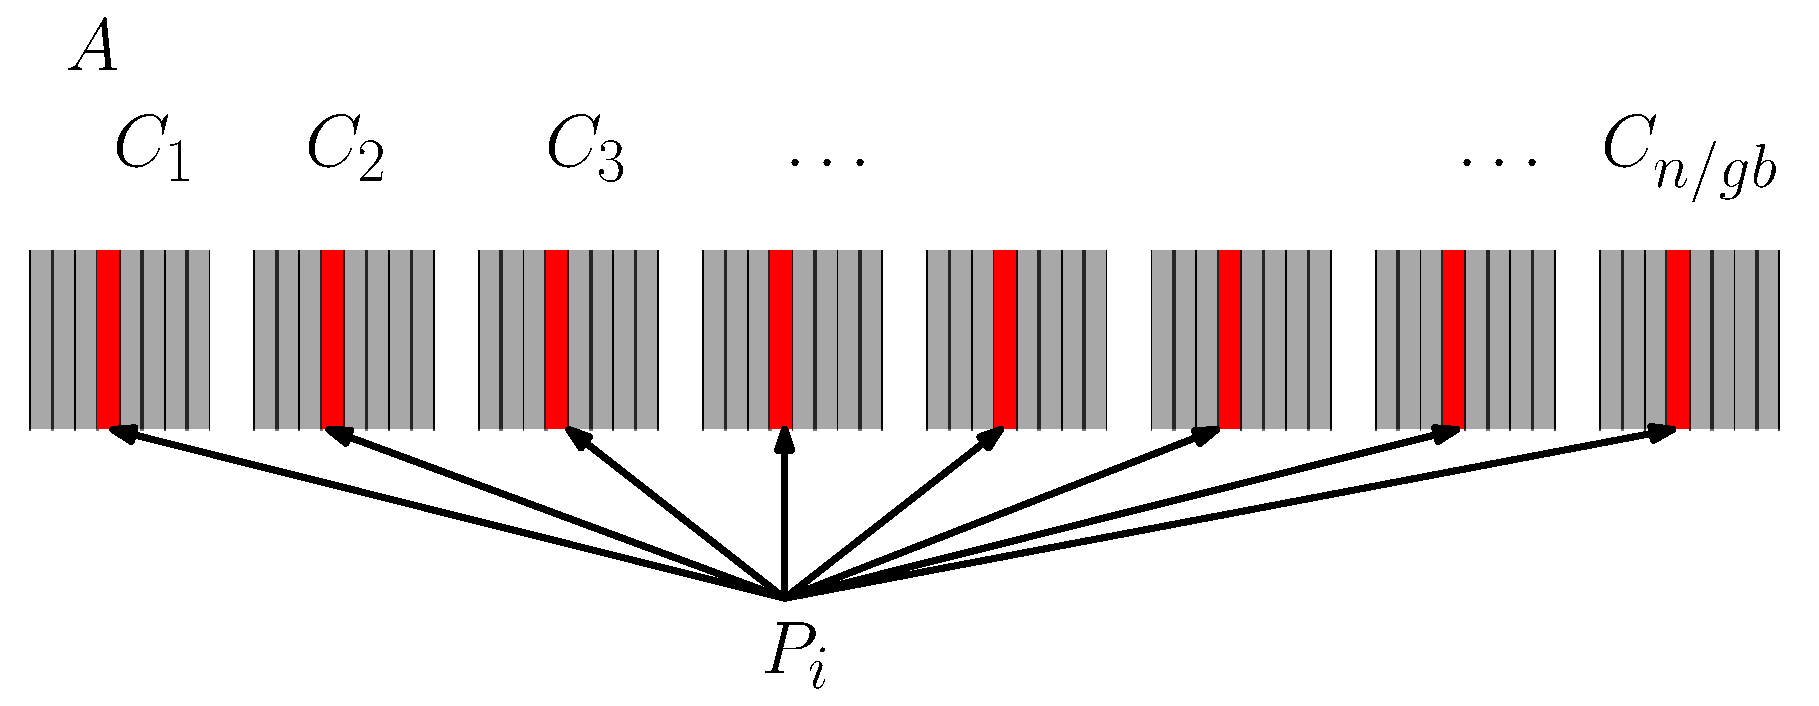
\includegraphics[width=\linewidth]{imgs/stridedAlgArrows.eps}
	\end{figure}
	% \begin{defin}[Partially Partitioned Array]
	%   $\exists u, l $ such that $$i < u \implies A[i] \text{ is predecessor }, i \ge l \implies A[i] \text{ is successor }$$
	% \end{defin}
	\begin{itemize}
		\item Logically partition $A_i$ into $P_i$ so that $P_i$ has the $i$-th block from each chunk $C_j$ of the array
		\item Perform serial partitions on all $P_i$ in parallel.
		\item Let $v_i$ be the position in $A$ of the first successor in $P_i$. Perform a serial partition on $A[\min_i v_i], \ldots, A[\max_i v_i -1]$.
	\end{itemize}
\end{frame}


\begin{frame}[t]{Strided Algorithm Analysis}
	\begin{itemize}
		\item Partial partition step: work $O(n)$, span $\Theta(n/g)$.
		\item Serial cleanup step: span $\Theta(v_\text{max}-v_\text{min})$, which is $O(n)$ in general.
		\item If the number of predecessors in each $P_i$ is similar, $v_\text{max}-v_\text{min}$ can be small.
		\item If array values are selected independently at random from some distribution, for appropriate choice of parameters, with high probability in $n$, the Strided Algorithm achieves span $$\tilde{O}(n^{2/3}),$$ and the number of cache misses is fewer than $$\frac{n}{b}+\frac{\tilde{O}(n^{2/3})}{b}.$$
		\item In particular, if $b\in \polylog(n)$, and the array values are selected independently at random from some distribution, and $g$ is chosen to optimize span ($g=n^{1/3}$), then with high probability in $n$, $$v_\text{max}-v_\text{min} < \tilde{O}(n^{2/3}),$$ the span is $$\tilde{O}(n^{2/3}),$$ and the number of cache misses is fewer than $$\frac{n}{b}+\frac{\tilde{O}(n^{2/3})}{b}.$$
	\end{itemize}
\end{frame}

\begin{frame}[t]{The Smoothed Striding Algorithm} 
	The Smoothed-Striding Algorithm creates groups analogous to the Strided Algorithm's $P_i$'s, but rather than taking the $i$-th element from each chunk of the array to form groups $P_i$, the Smoothed-Striding algorithm takes a random element from each chunk for each of the groups $U_i$.

	\textbf{Blocked Strided Algorithm $P_i$.}
	\begin{figure}
		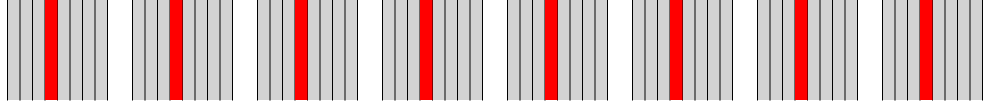
\includegraphics[width=\linewidth]{imgs/stridedAlgHighlighted.png}
	\end{figure}
	\textbf{Smoothed-Striding Algorithm $U_i$.}
	\begin{figure}
		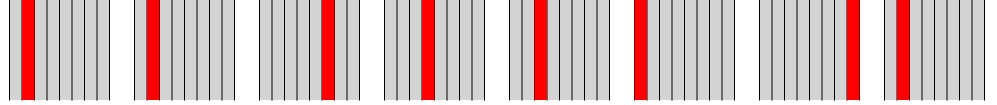
\includegraphics[width=\linewidth]{imgs/smoothedStridingAlgHighlighted.png}
	\end{figure}
\end{frame}



% \begin{frame}[t]{}%{Strided Algorithm Description}
	\vspace{0.25cm}
	\begin{overprint}
	\onslide<1>Logically partition the array into chunks of adjacent elements:
	\onslide<2>Form groups $P_i$ where $P_i$ contains the $i$-th element from each chunk:
	\onslide<3>Perform serial partitions on each $P_i$ in parallel over the $P_i$'s:
	\onslide<4>Identify the splitting index $v_i$ (the first element greater than the pivot) of each $P_i$. 
	\onslide<5>Partition the subarray from the minimum splitting index to the maximum splitting index in serial. This completes the partition. 
	\end{overprint}
	\vspace{0.25cm}
	\begin{overprint}
	\onslide<1>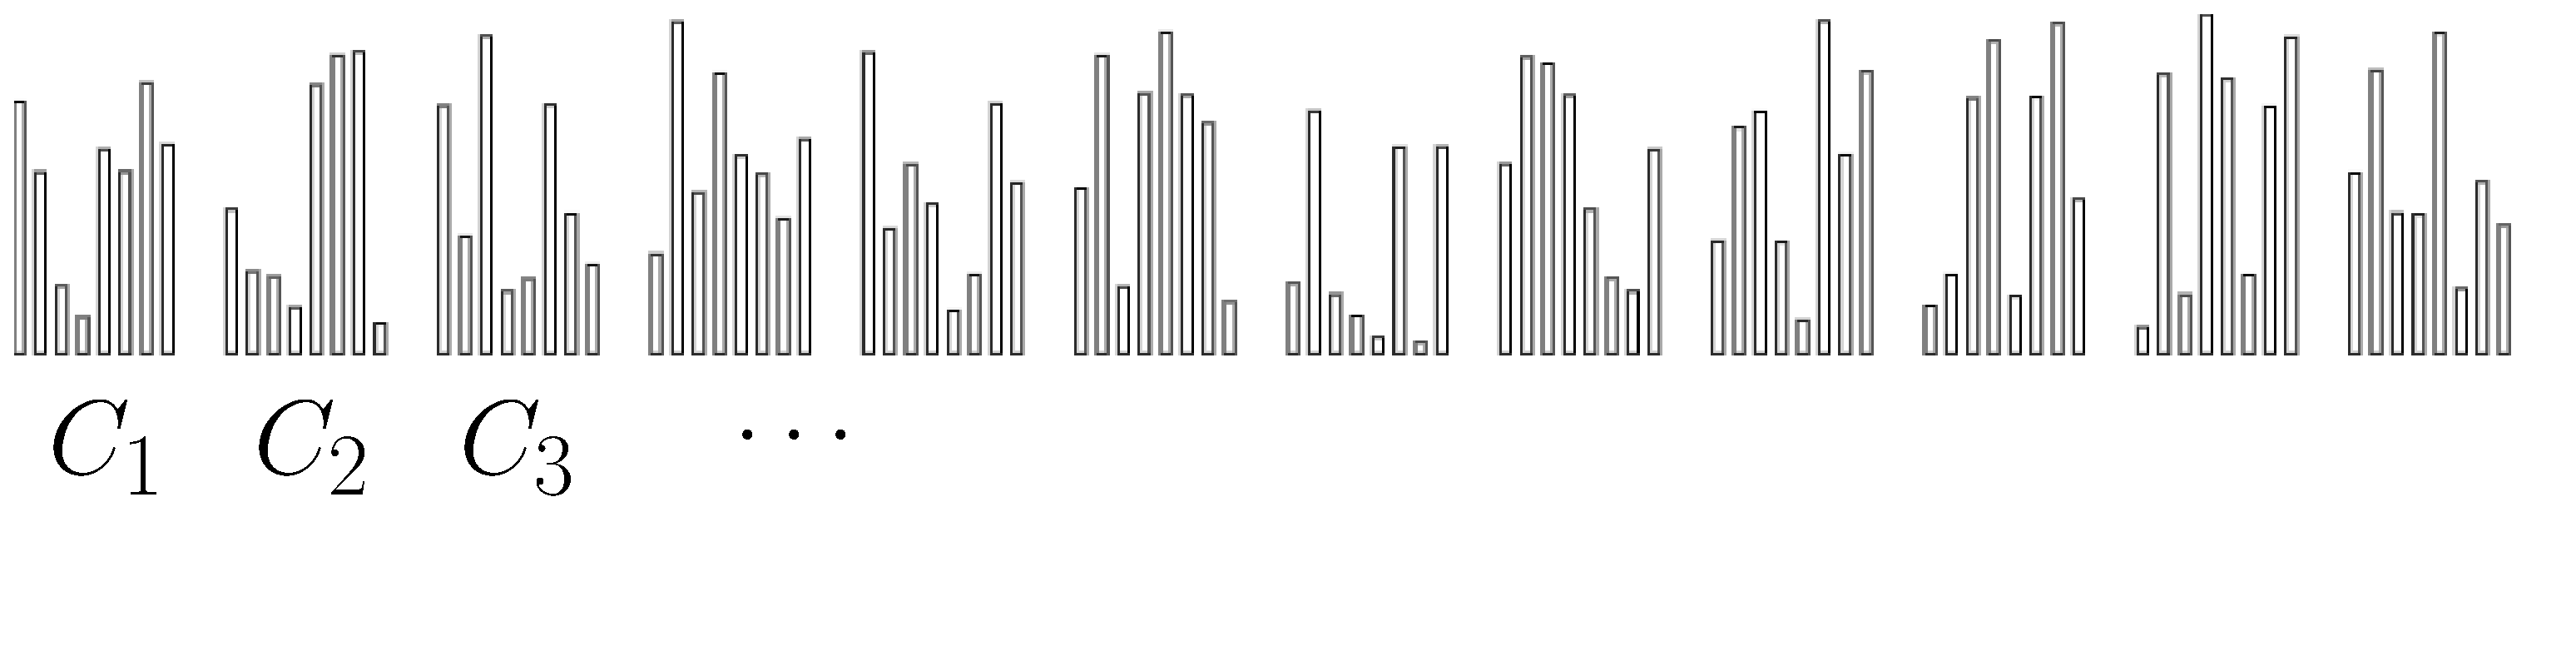
\includegraphics[width=\linewidth]{imgs/oldStridedAlgSim/stridedAlgSim1Ann.eps}
	\onslide<2>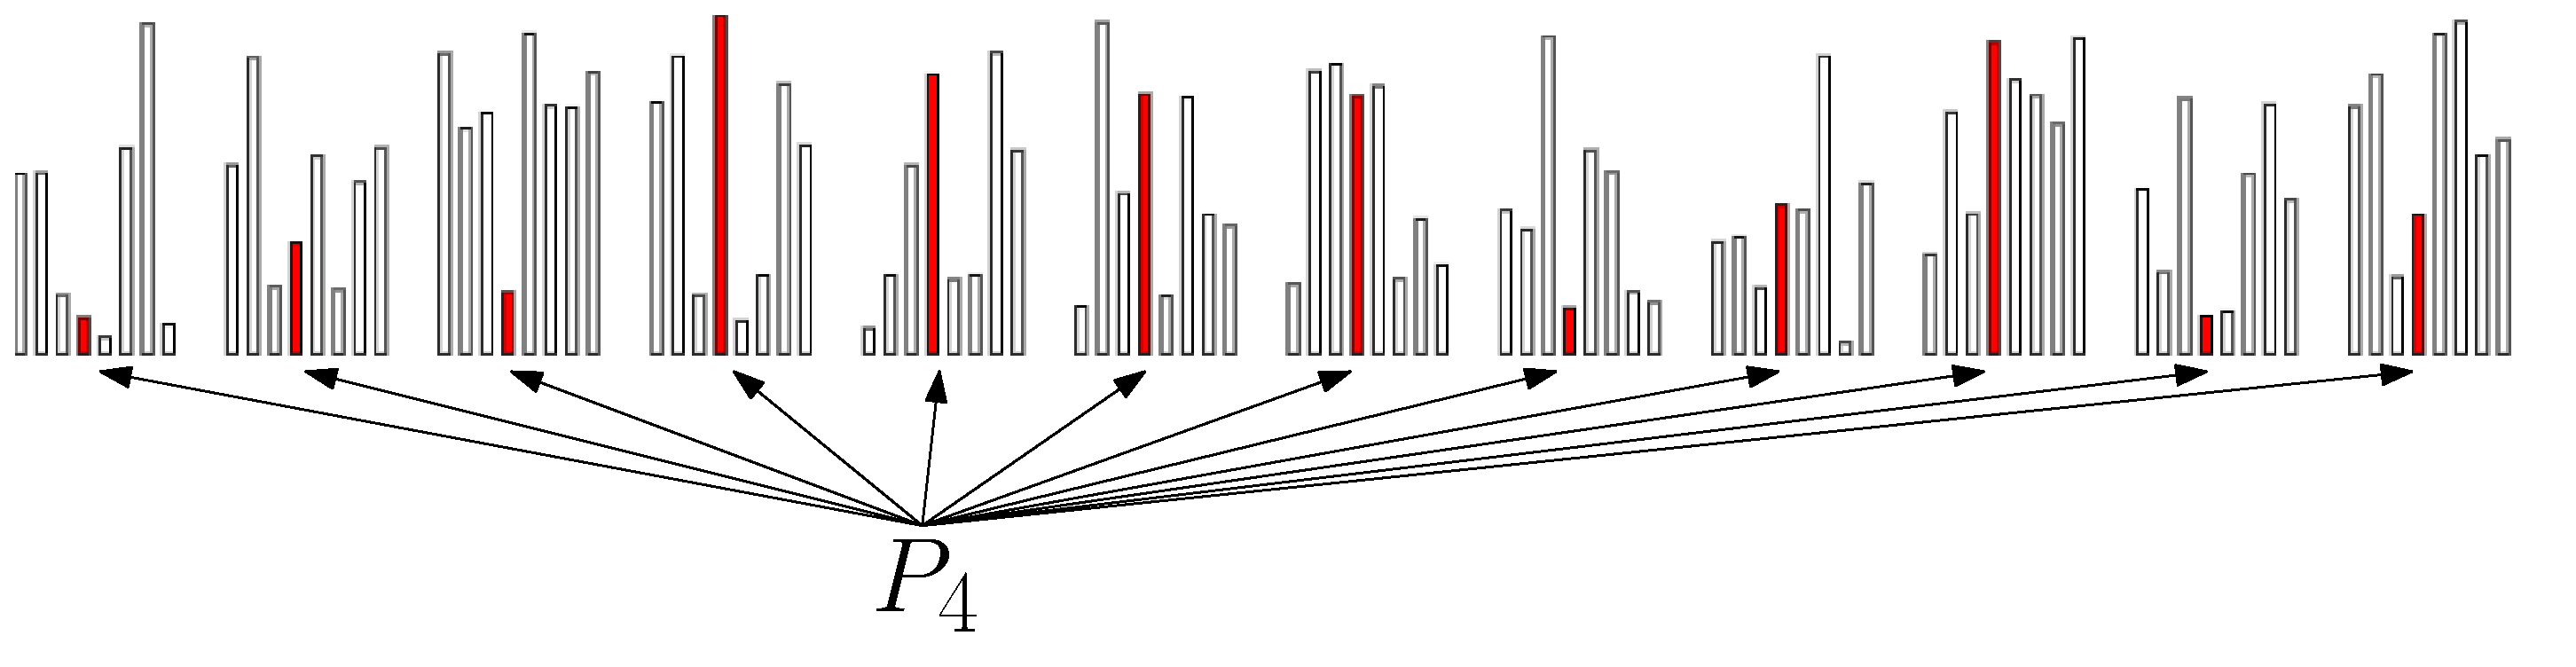
\includegraphics[width=\linewidth]{imgs/oldStridedAlgSim/stridedAlgSim2Ann.eps}
	\onslide<3>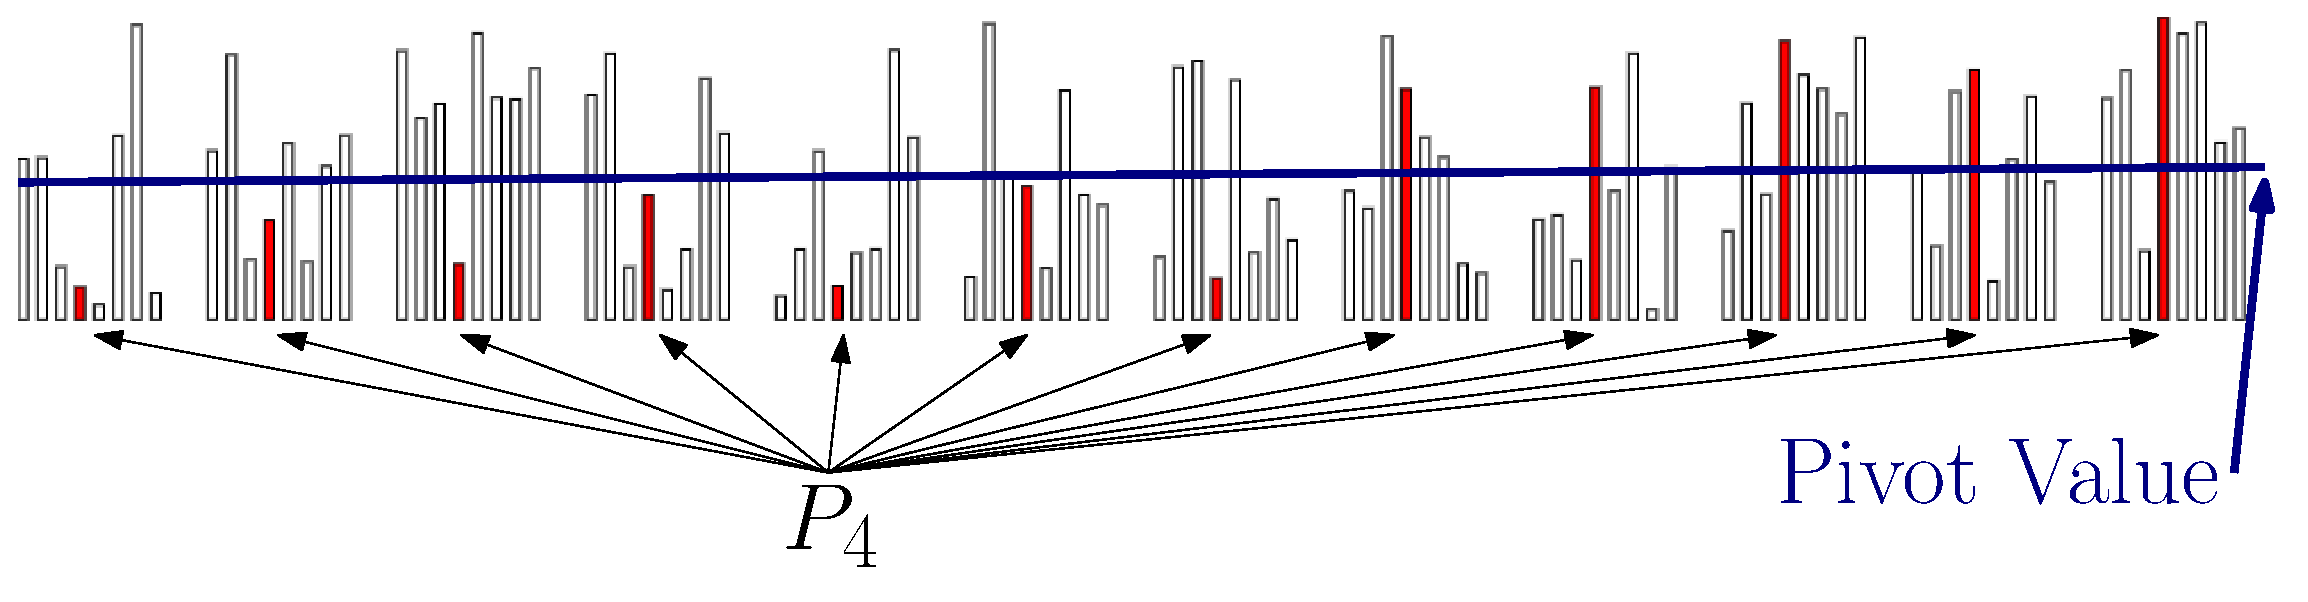
\includegraphics[width=\linewidth]{imgs/oldStridedAlgSim/stridedAlgSim3Ann.eps}
	\onslide<4>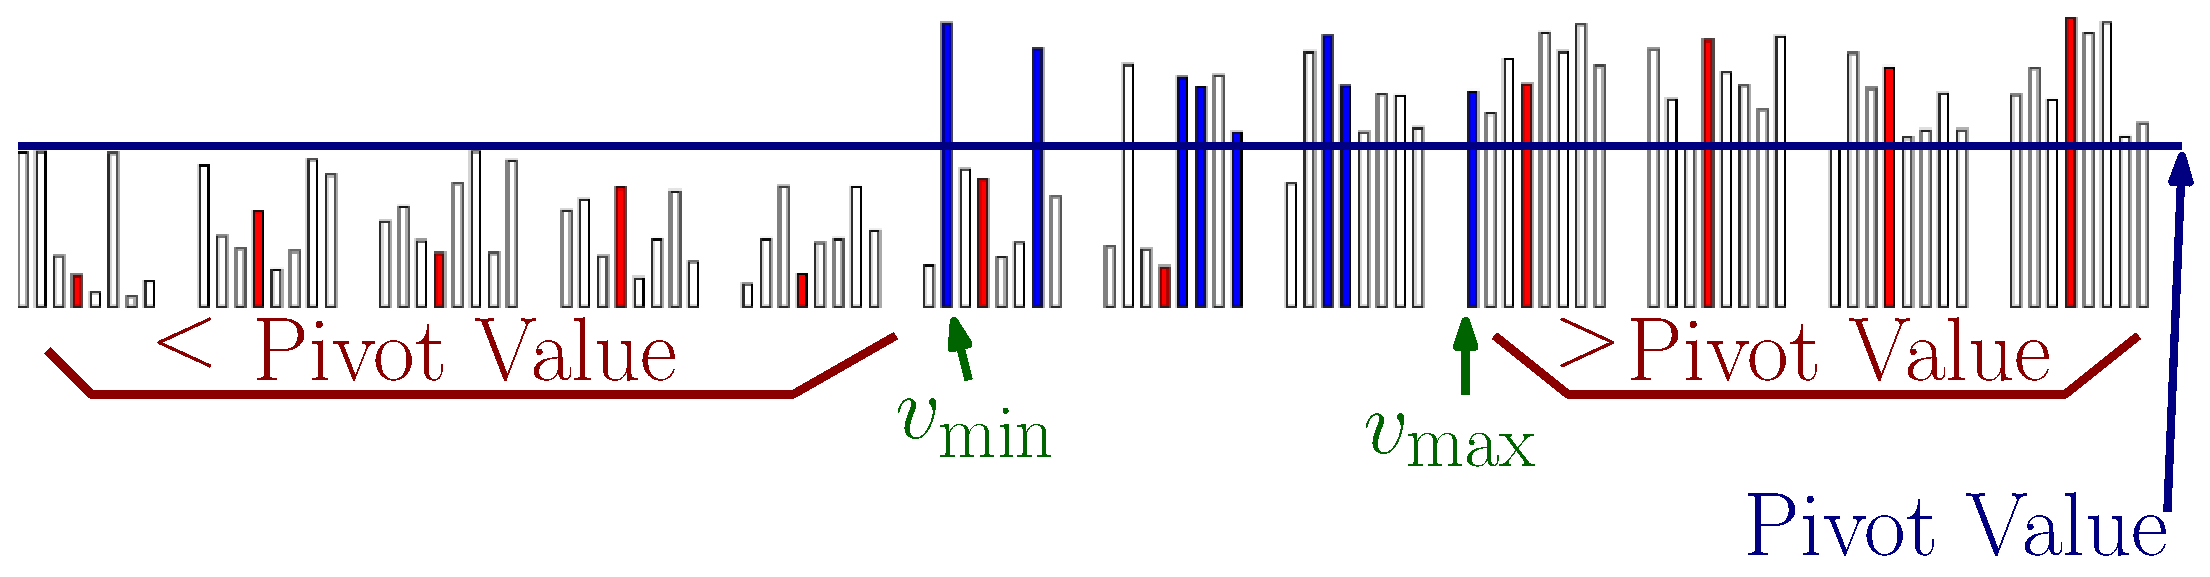
\includegraphics[width=\linewidth]{imgs/oldStridedAlgSim/stridedAlgSim4Ann.eps}
	\onslide<5>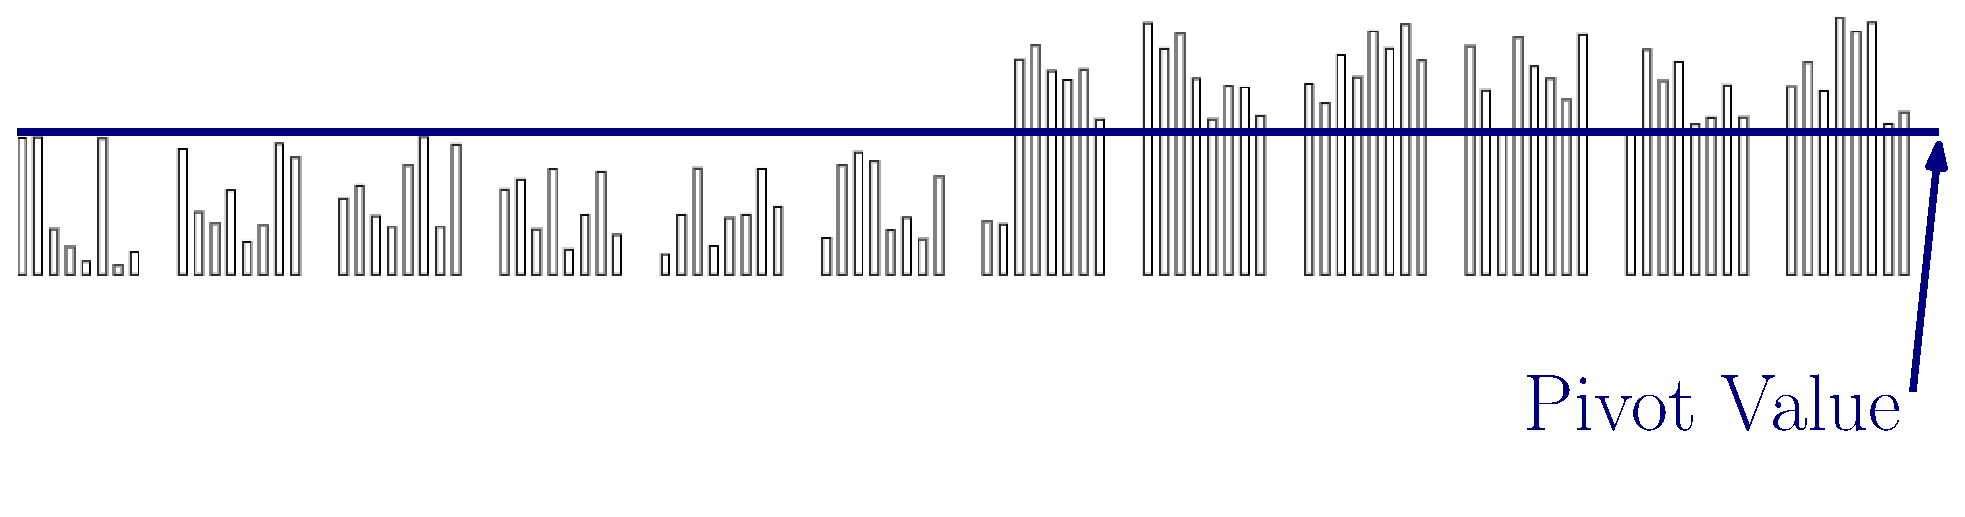
\includegraphics[width=\linewidth]{imgs/oldStridedAlgSim/stridedAlgSim5Ann.eps}
	\end{overprint}
	\vspace{0.25cm}
	\begin{overprint}
	\onslide<3>This step is highly parallel.
	% \onslide<4>Note that all elements below the minimum splitting index are less than the pivot and all elements greater than the maximum splitting index are greater than the pivot.
	\onslide<5> Note that this step has no parallelism. In general this results in span $O(n)$. However, if the number of elements less than the pivot in each $P_i$ is similar, then size of the subarray to be partitioned can be very small.
	\end{overprint}
\end{frame}

\begin{frame}[t]{}%{Smoothed Striding Algorithm Description}
	\vspace{0.25cm}
	\begin{overprint}
	\onslide<1>Logically partition the array into chunks of adjacent elements:
	\onslide<2>Form groups $U_i$ where $U_i$ contains the $i$-th element from each chunk:
	\onslide<3>Perform serial partitions on each $U_i$ in parallel over the $U_i$'s:
	\onslide<4>Identify the splitting index $v_i$ (the first element greater than the pivot) of each $P_i$. 
	\onslide<5>Recursively apply this algorithm to partition the subarray from the minimum splitting index to the maximum splitting index in serial. This completes the partition. 
	\end{overprint}
	\vspace{0.25cm}
	\begin{overprint}
	\onslide<1>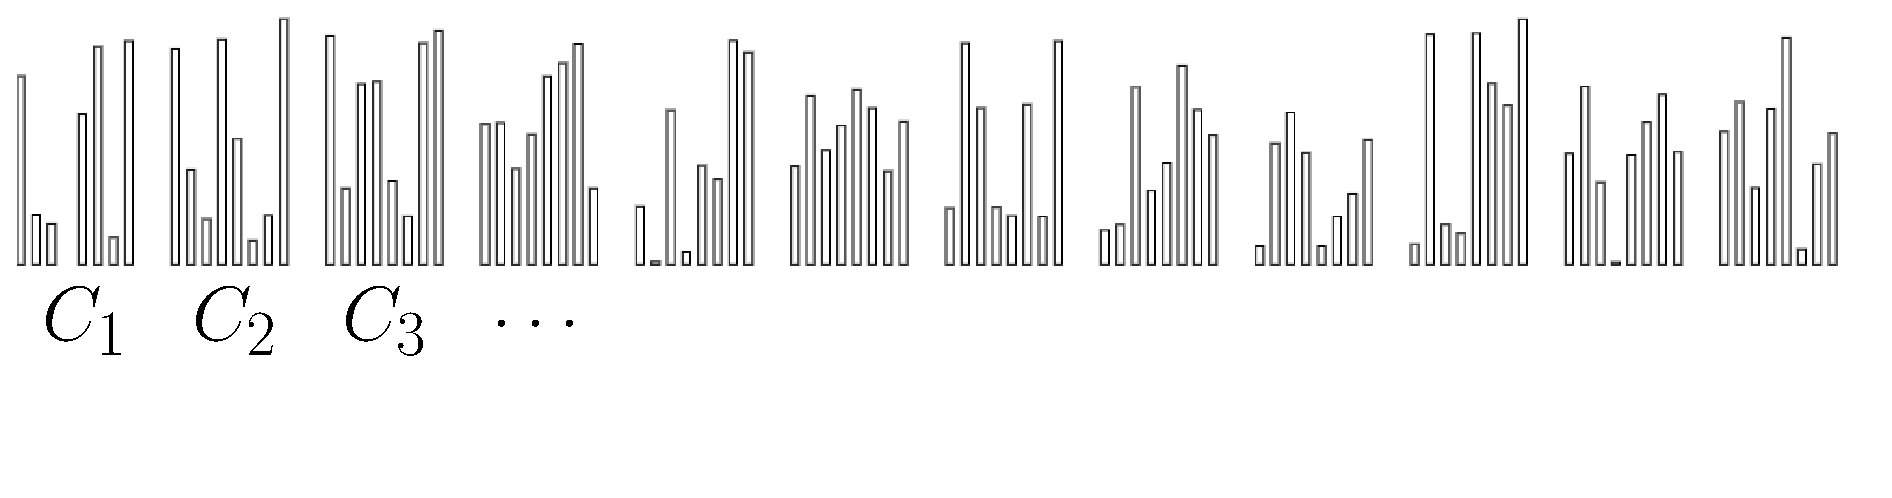
\includegraphics[width=\linewidth]{imgs/smoothedAlgSim1Ann.eps}
	\onslide<2>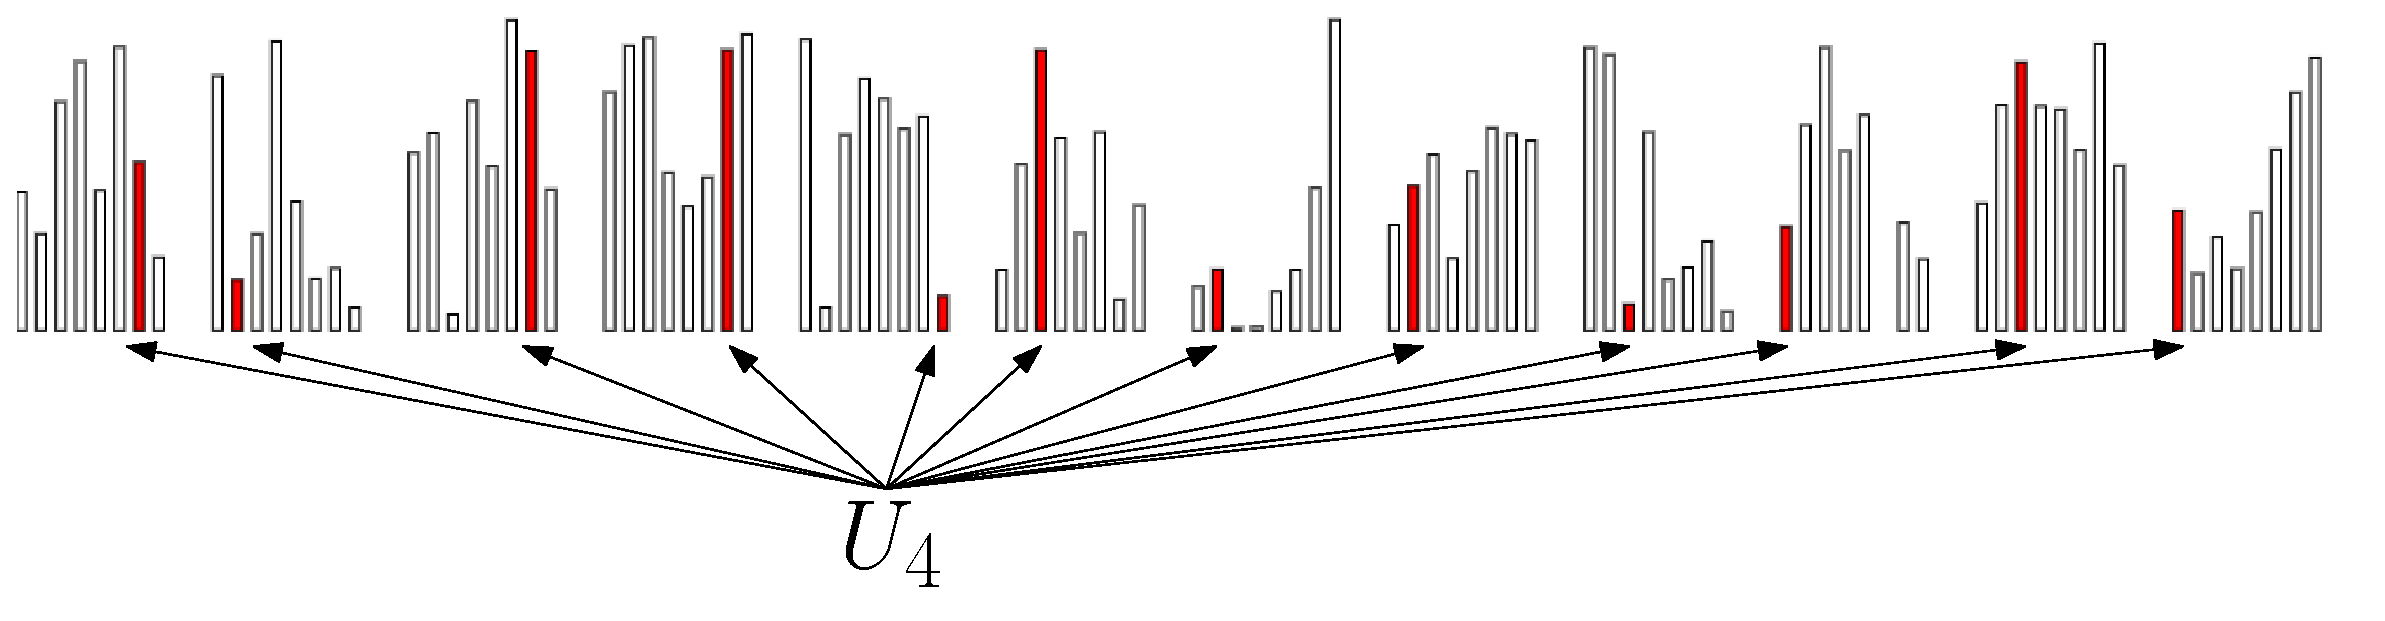
\includegraphics[width=\linewidth]{imgs/smoothedAlgSim2Ann.eps}
	\onslide<3>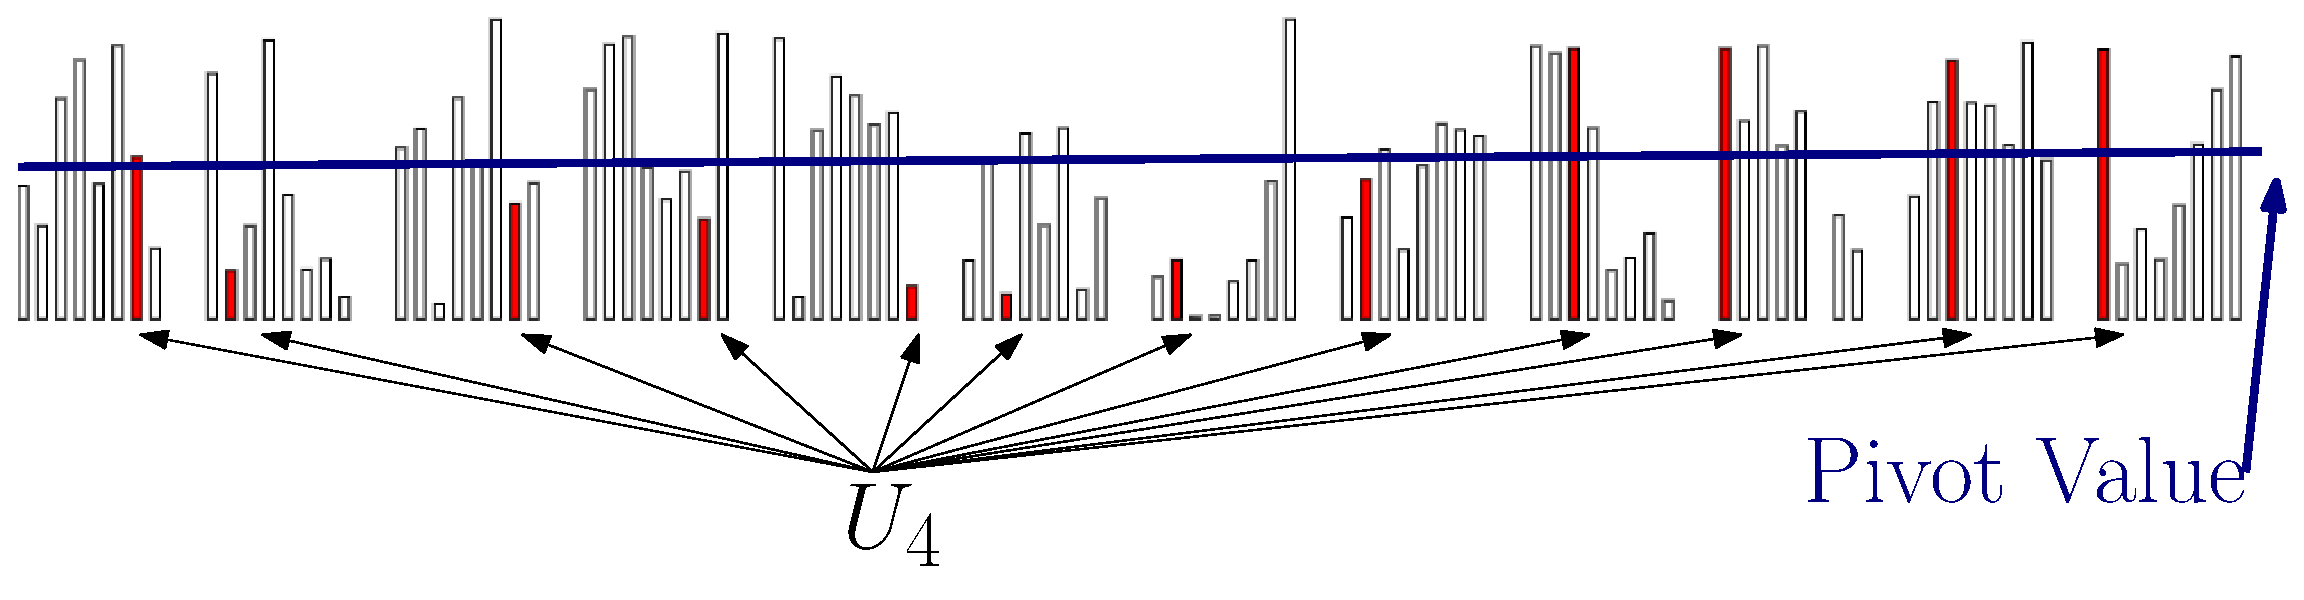
\includegraphics[width=\linewidth]{imgs/smoothedAlgSim3Ann.eps}
	\onslide<4>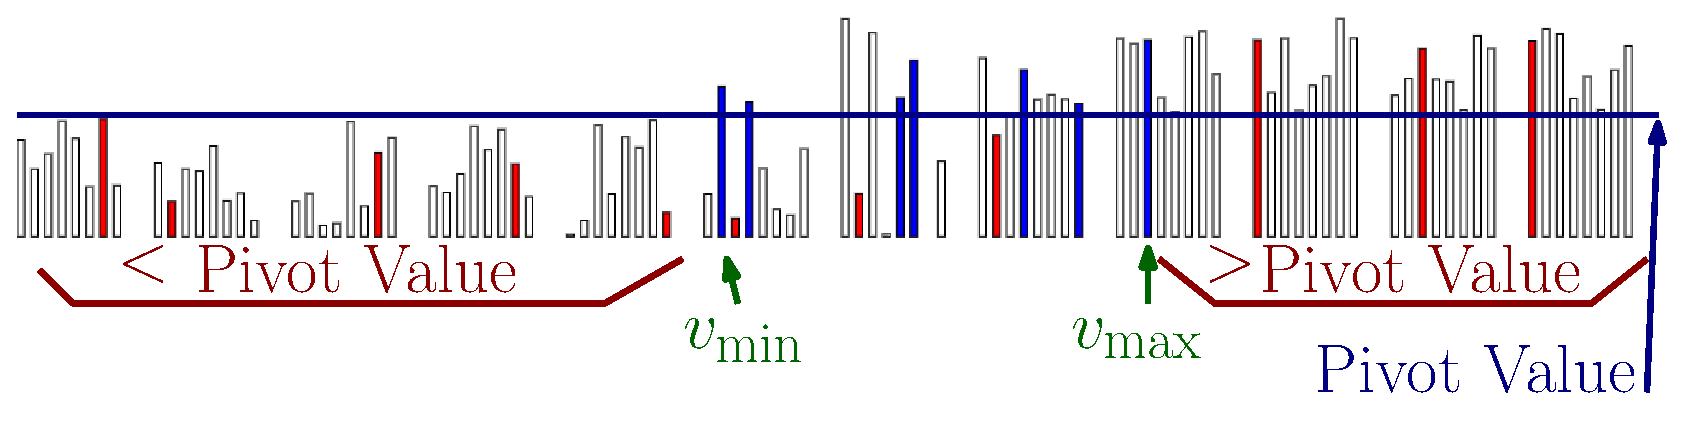
\includegraphics[width=\linewidth]{imgs/smoothedAlgSim4Ann.eps}
	\onslide<5>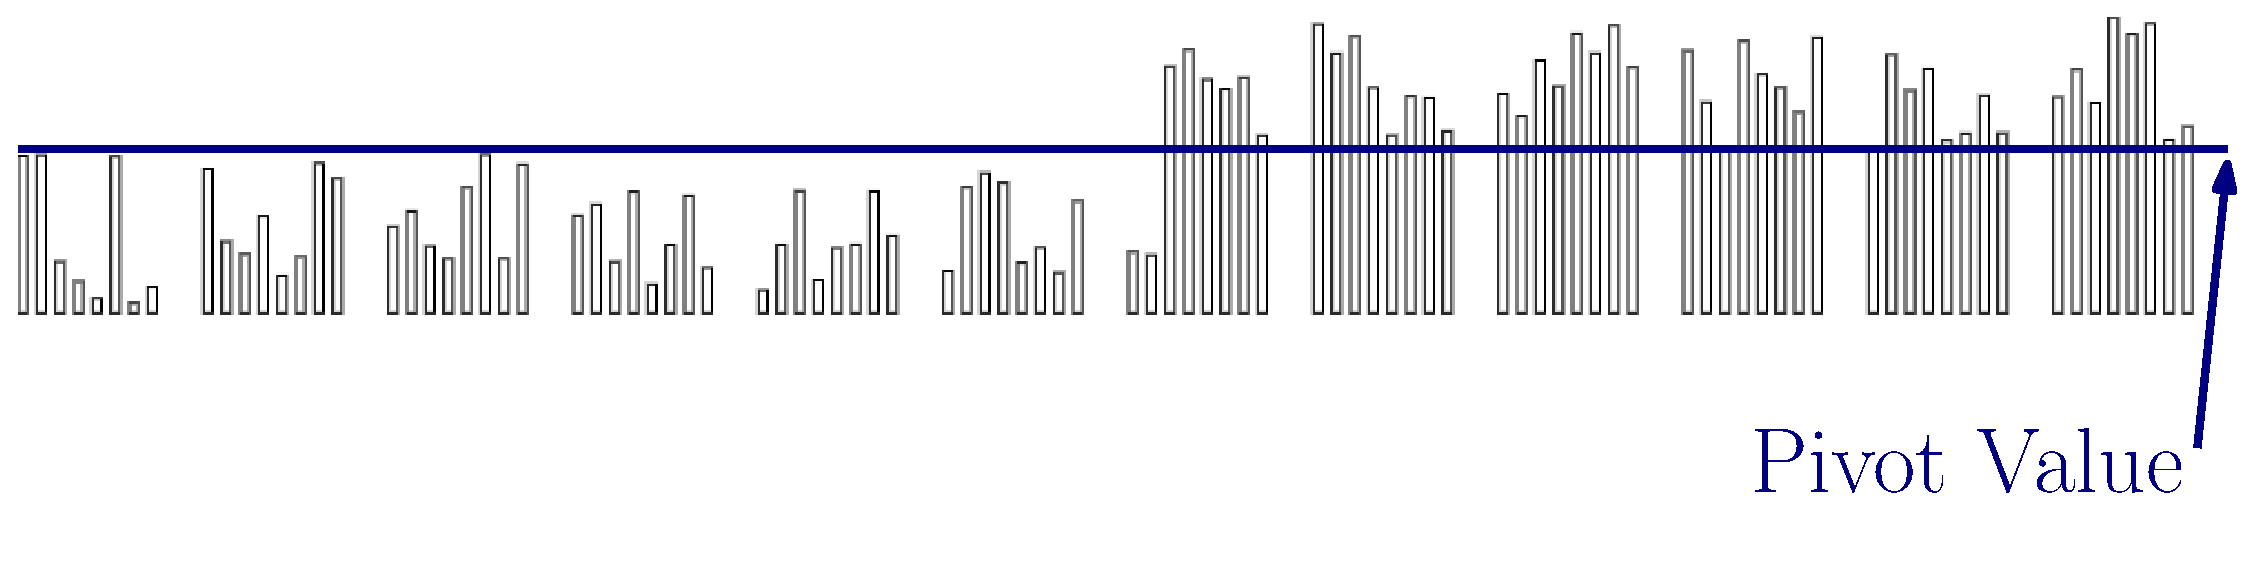
\includegraphics[width=\linewidth]{imgs/smoothedAlgSim5Ann.eps}
	\end{overprint}
	\vspace{0.25cm}
	\begin{overprint}
	\onslide<3>This step is highly parallel.
	% \onslide<4>Note that all elements below the minimum splitting index are less than the pivot and all elements greater than the maximum splitting index are greater than the pivot.
	\onslide<5>Unlike in the Strided Algorithm this step has parallelism, and is guaranteed to only run on a small subarray. The Strided Algorithm could not recurse here because the subproblem is a worst case input for it.
	\end{overprint}
\end{frame}

\end{document}
